% !TEX root = SPP2.tex
\section{Numerical Simulations \label{sec:sim}}
We demonstrate our proposed methods using a four-vehicle example. Each vehicle has the following model:
\vspace{-0.2em}
\begin{equation*}
\label{eq:dyn_i}
\begin{aligned}
\dot{\pos}_{x,i} &= v_i \cos \theta_i + d_{x,i} &\\
\dot{\pos}_{y,i} &= v_i \sin \theta_i + d_{y,i} & \underline{v} \le v_i \le \bar{v}, |\omega_i| \le \bar{\omega}\\
\dot{\theta}_i &= \omega_i + d_{\theta,i} & \|(d_{x,i}, d_{y,i}) \|_2 \le d_{r}, |d_{\theta,i}| \le \bar{d_{\theta}}\\
\end{aligned}
\end{equation*}

\noindent where $p_i = (p_{x,i}, p_{y,i}), \theta_i, d = (d_{x,i}, d_{y,i}, d_{\theta,i})$ respectively represent $\veh_i$'s position, heading, and disturbances in the three states. The control of $\veh_i$ is $u_i = (v_i, \omega_i)$, where $v_i$ is the speed of $\veh_i$ and $\omega_i$ is the turn rate; both controls have a lower and upper bound. For illustration purposes, we choose $\underline{v} = 0.5, \bar{v} = 1, \bar\omega = 1$; however, our method can easily handle the case in which these inputs differ across vehicles and cases in which each vehicle has a different dynamic model. The disturbance bounds are chosen as $d_{r} = 0.1, \bar{d_{\theta}} = 0.2$, which correspond to a 10\% uncertainty in the dynamics. %The optimal control for vehicle $i$ can be obtained by optimizing the associated Hamiltonian, $H_i(t, D_{\bm{x}_i} V_i(\bm{x}_i,t), V_i(\bm{x}_i,t))$, and is given by:

%\begin{equation}
%\omega_i(t) = -\bar{\omega}_i \frac{D_{\theta_i}V_i(\bm{x}_i,t)}{\left| D_{\theta_i}V_i(\bm{x}_i,t) \right|},
%\end{equation}
%
%\begin{equation}
%v_i(t) =
%\left \{ 
%\begin{array}{ll}
%\underline{v} & \mbox{ if } D_{x_i}V_i(\bm{x}_i,t) \cos \theta_i + D_{y_i}V_i(\bm{x}_i,t) \sin \theta_i \geq 0 \\
%\bar{v} & \mbox{ otherwise } 
%\end{array}
%\right.
%\end{equation}

The initial states of the vehicles are given as follows:
\begin{equation}
\begin{aligned}
x_1^0 &= (-0.5, 0, 0), \quad &x_2^0 = (0.5, 0, \pi), \\
x_3^0 &= \left(-0.6, 0.6, 7\pi/4\right), \quad &x_4^0 = \left(0.6, 0.6, 5\pi/4\right).
\end{aligned}
\end{equation}

\noindent Each of the vehicles has a target set $\targetset_i$ that is circular in their position $\pos_i$ centered at $c_i = (c_{x,i}, c_{y,i})$ with radius $r$:
\vspace{-0.2em}
\begin{equation}
\targetset_i = \{x_i \in \R^3: \|p_i - c_i\| \le r\}
\end{equation}

\noindent For the example shown, we chose $c_1 = (0.7, 0.2), c_2 = (-0.7, 0.2), c_3 = (0.7, -0.7), c_4 = (-0.7, -0.7)$ and $r = 0.1$. The setup of the example is shown in Fig. \ref{fig:initSetup}.

Using the SPP algorithms presented, we obtain $\ldt_i, i=1,2,3,4$ assuming $\sta_i=0$. Note that even though $\sta_i$ is assumed to be same for all vehicles in this example for simplicity, our method can easily handle the case in which $\sta_i$ is different for each vehicle.

For each proposed method of computing induced obstacles, we show the vehicles' entire trajectories (colored dotted lines), and overlay their positions (colored asterisks) and headings (arrows) at a point in time in which they are in relatively dense configuration. In all cases, the vehicles are able to avoid each other's danger zones (colored dashed circles) while getting to their target sets in minimum time. In addition, we show the evolution of the BRS over time for $\veh_3$ (green boundaries) as well as the obstacles induced by the higher-priority vehicles (black boundaries).

\begin{figure}[t!]
\centering
\begin{subfigure}{.35\columnwidth}
  \centering
  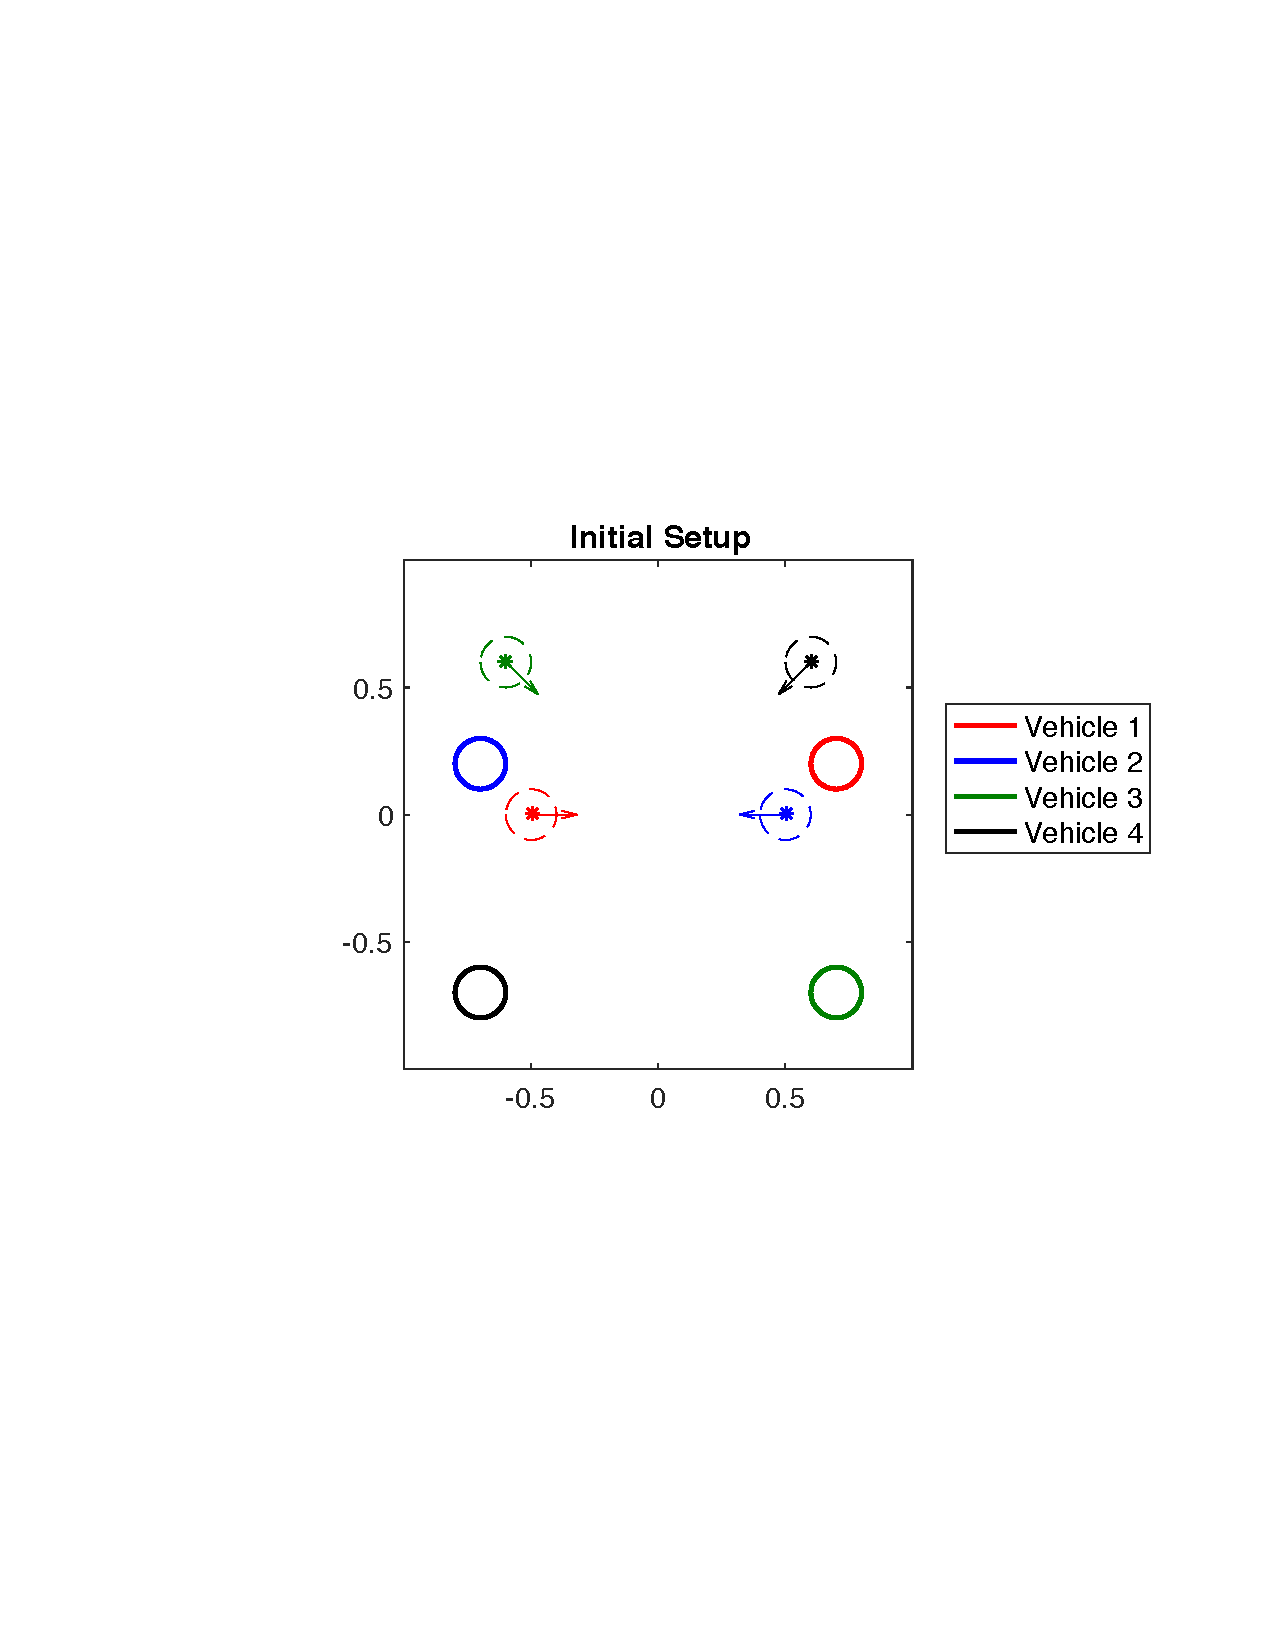
\includegraphics[width=\columnwidth]{fig/init_setup}
  \subcaption{}
  \label{fig:initSetup}
\end{subfigure}%
\begin{subfigure}{.35\columnwidth}
  \centering
  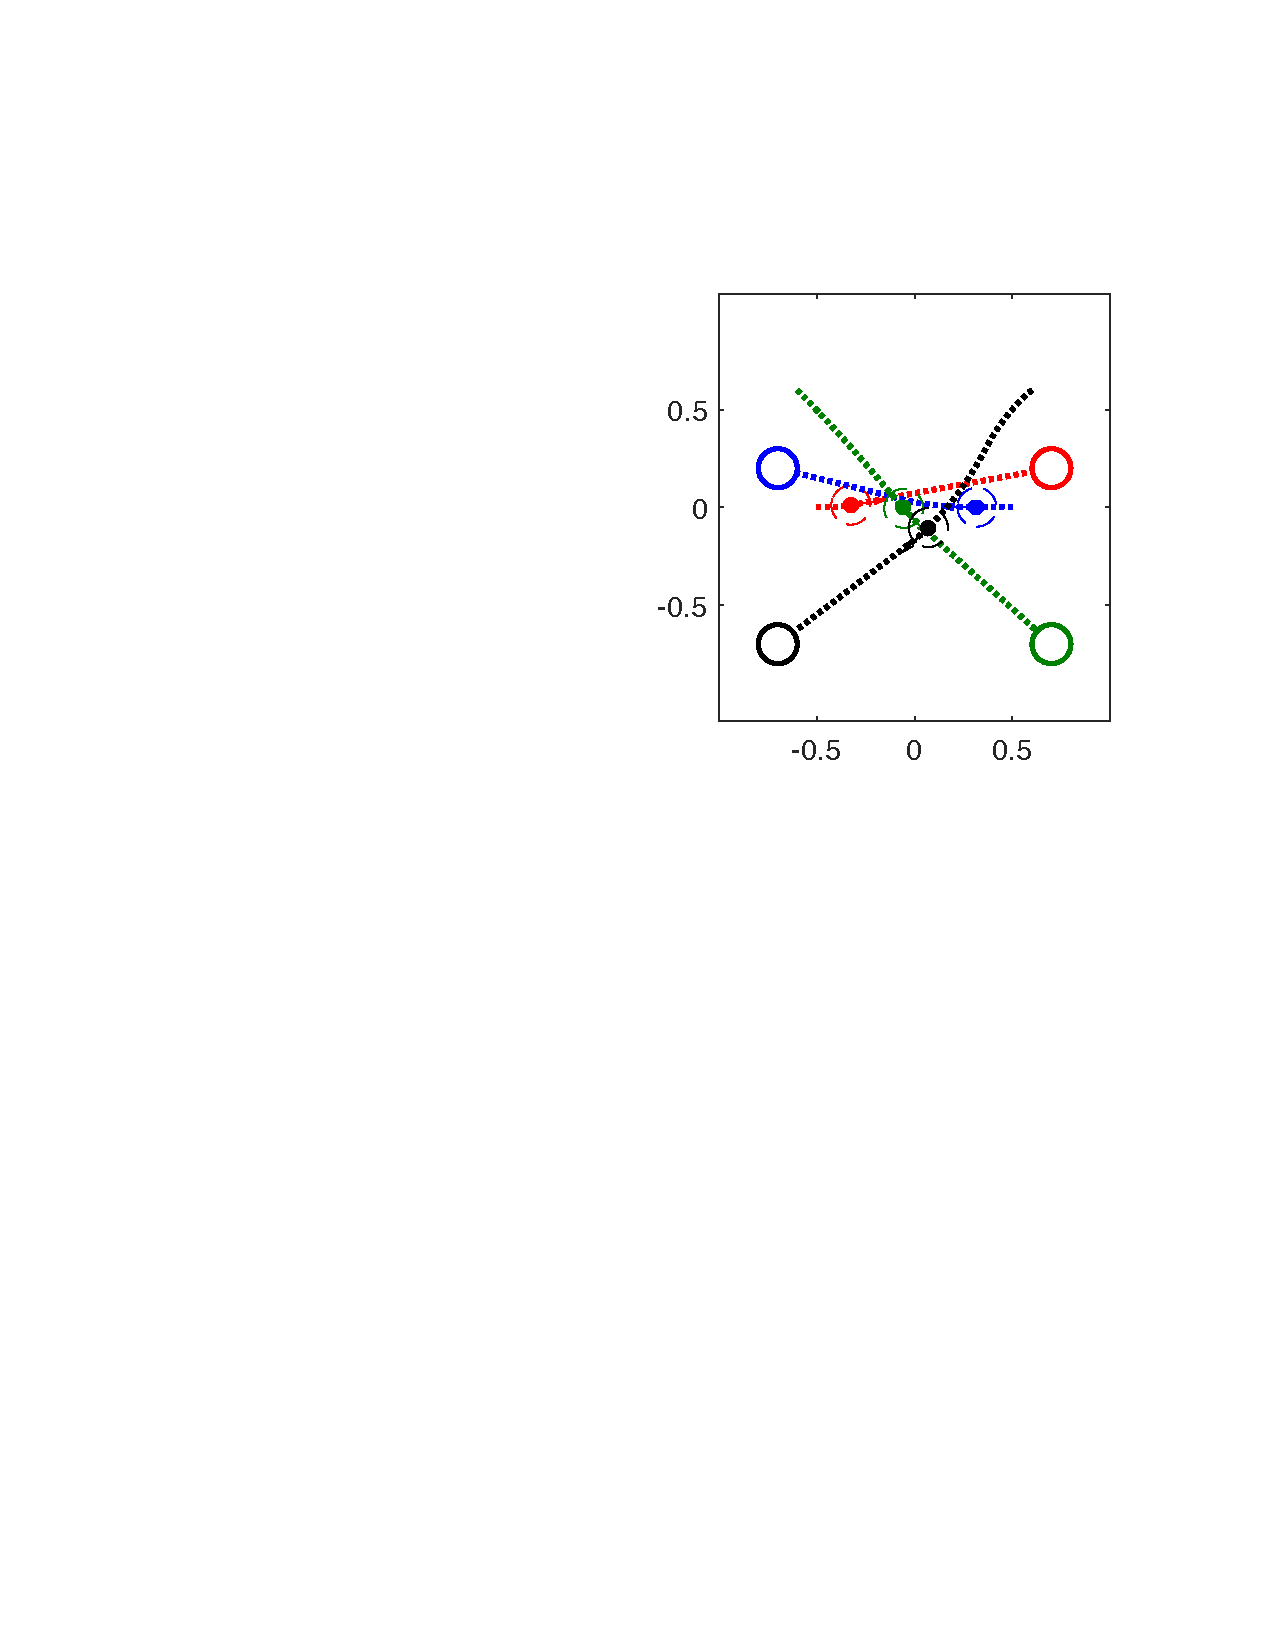
\includegraphics[width=\columnwidth]{fig/cc_trajs}
  \subcaption{}
  \label{fig:trajsCC}
\end{subfigure}
\begin{subfigure}{.35\columnwidth}
  \centering
  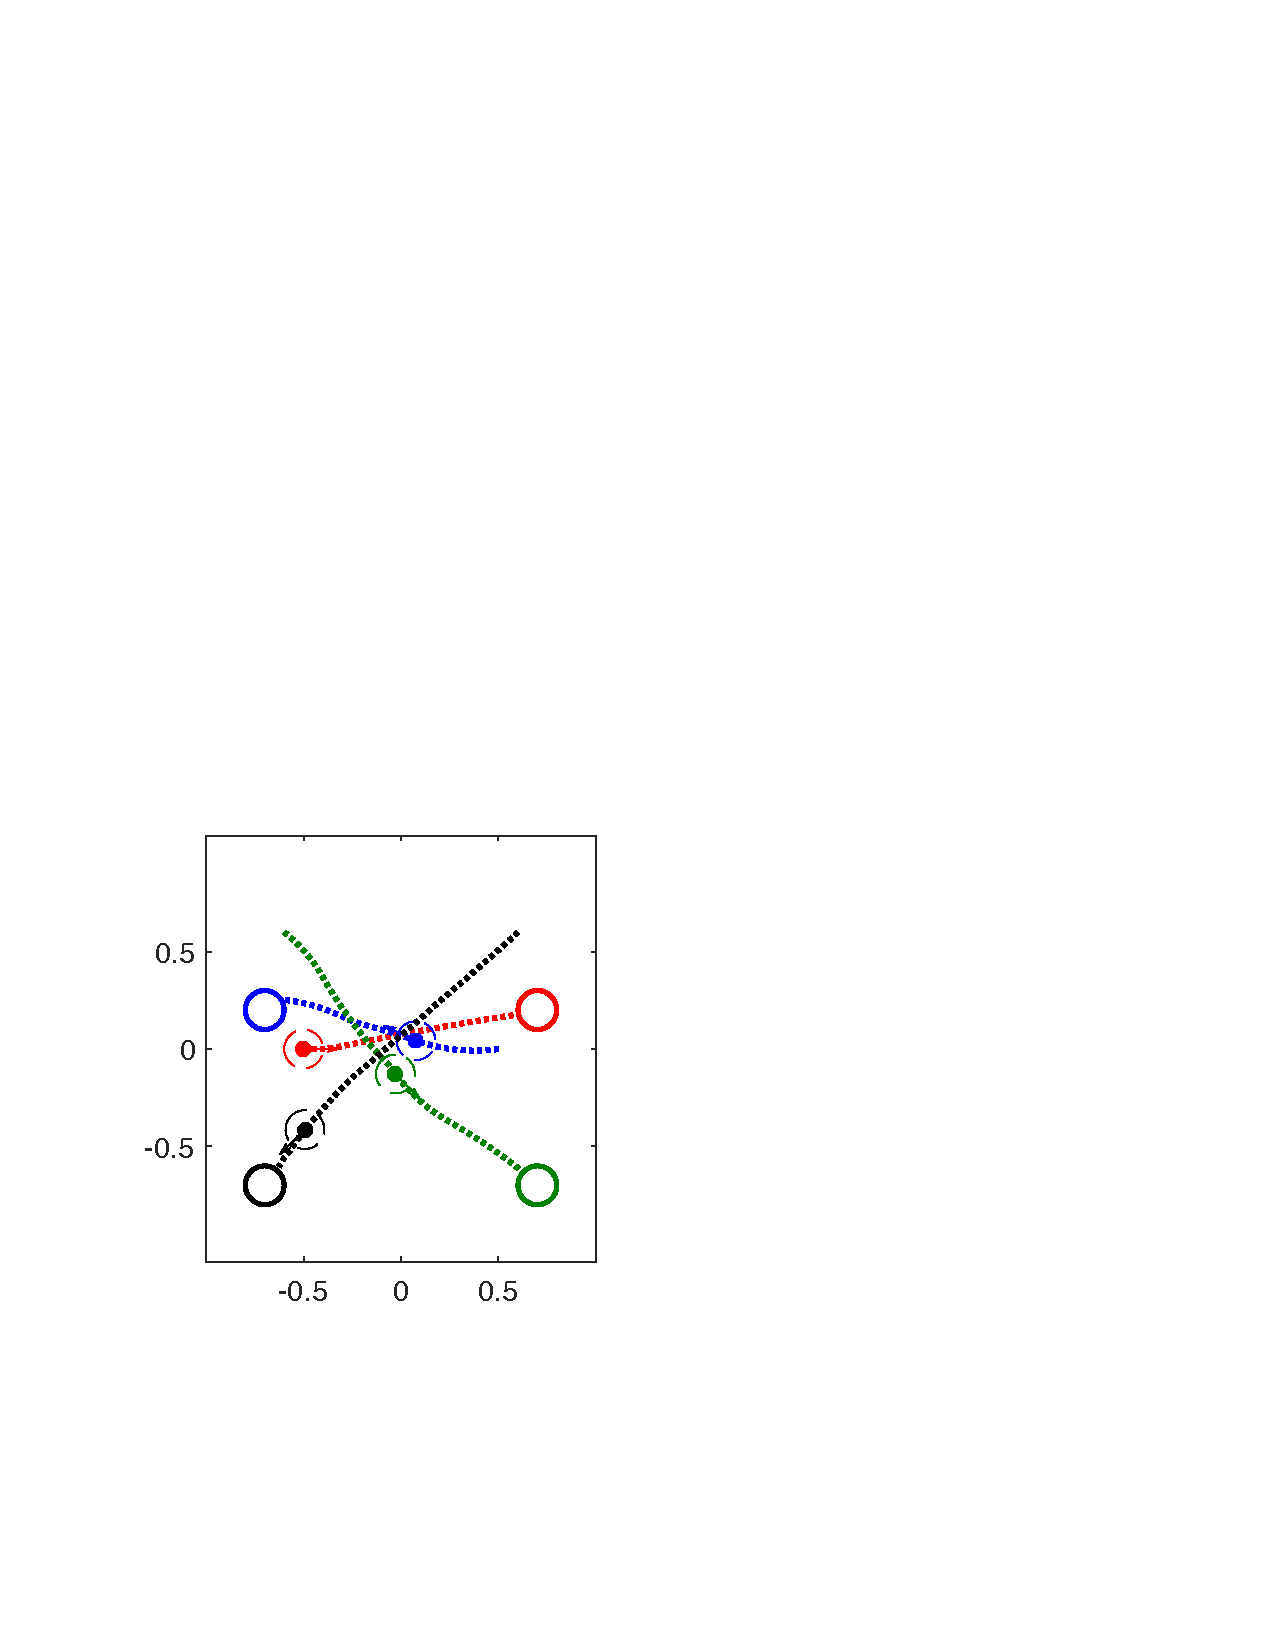
\includegraphics[width=\columnwidth]{fig/lrc_trajs}
  \subcaption{}
  \label{fig:trajsLRC}
\end{subfigure}
\begin{subfigure}{.35\columnwidth}
  \centering
  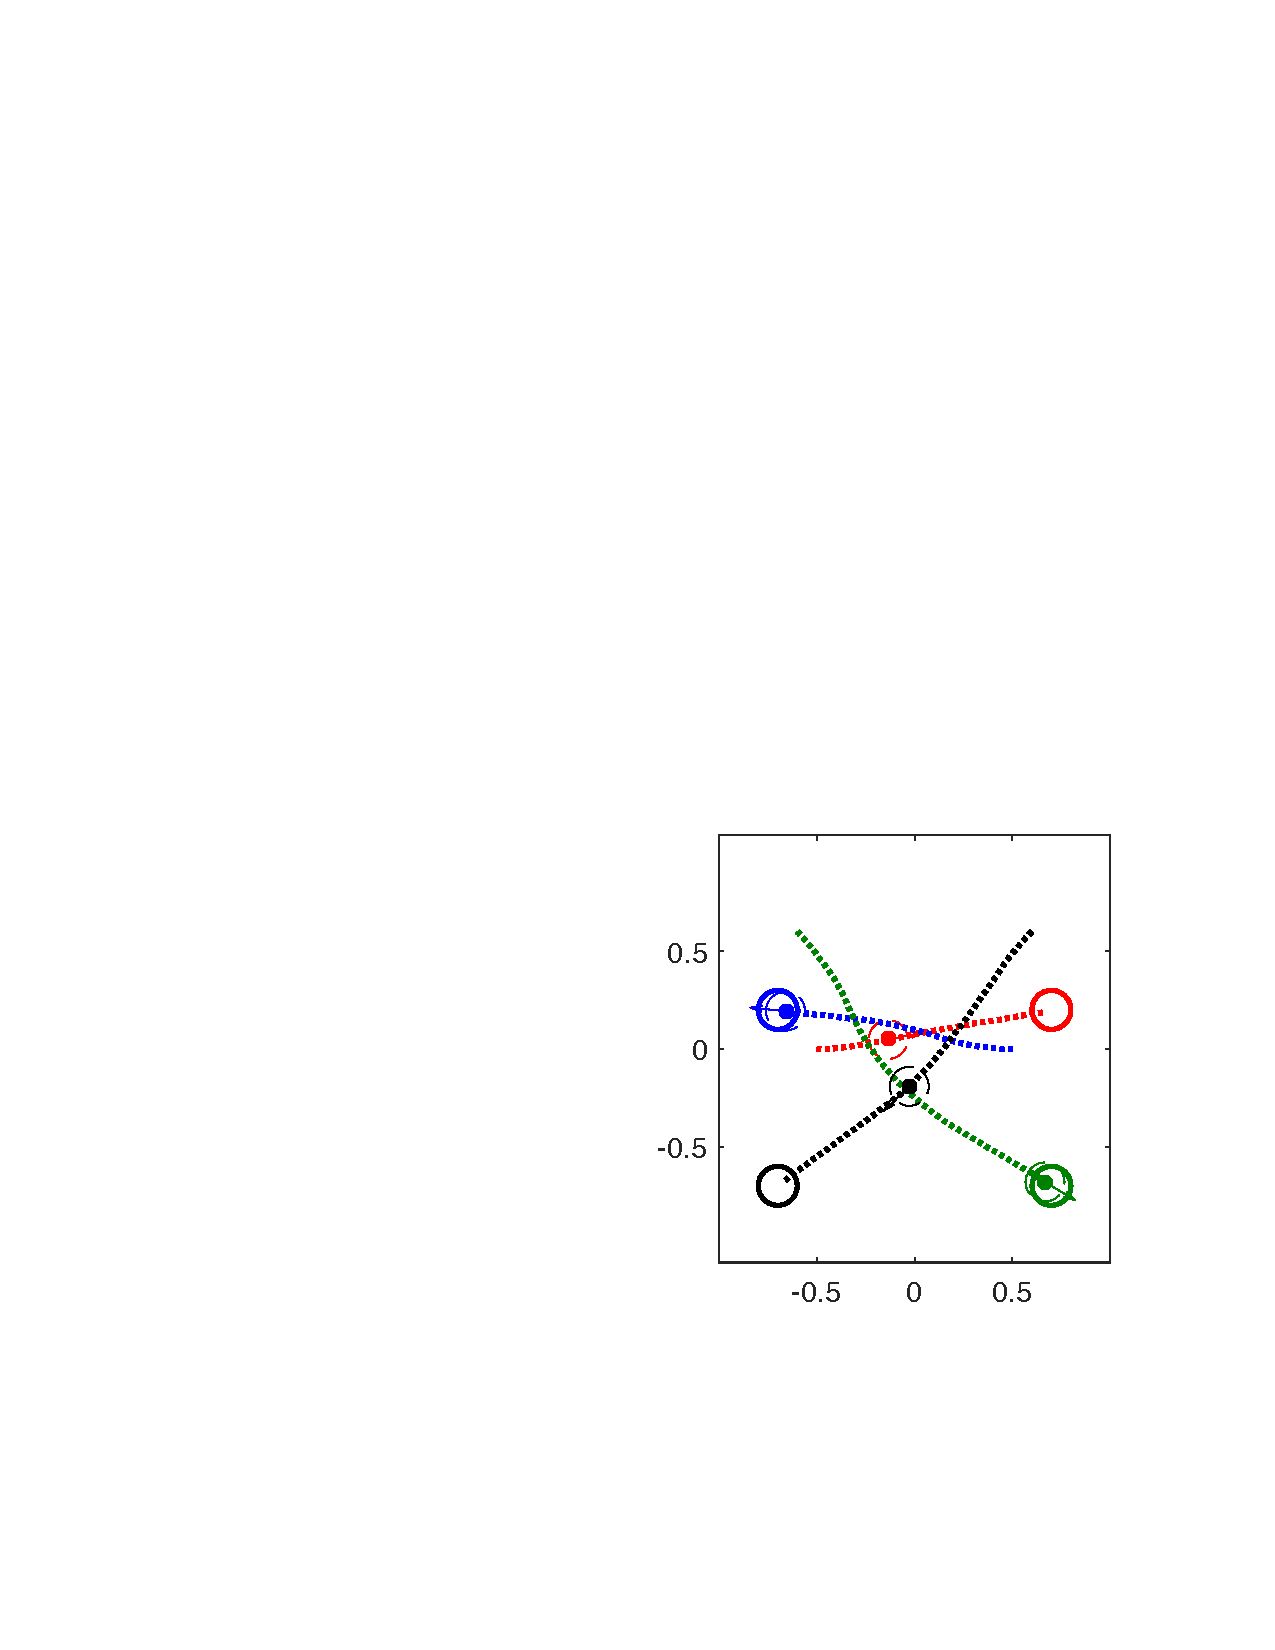
\includegraphics[width=\columnwidth]{fig/rtt_trajs}
  \subcaption{}
  \label{fig:trajsRTT}
\end{subfigure}
\begin{subfigure}{.7\columnwidth}
  \centering
  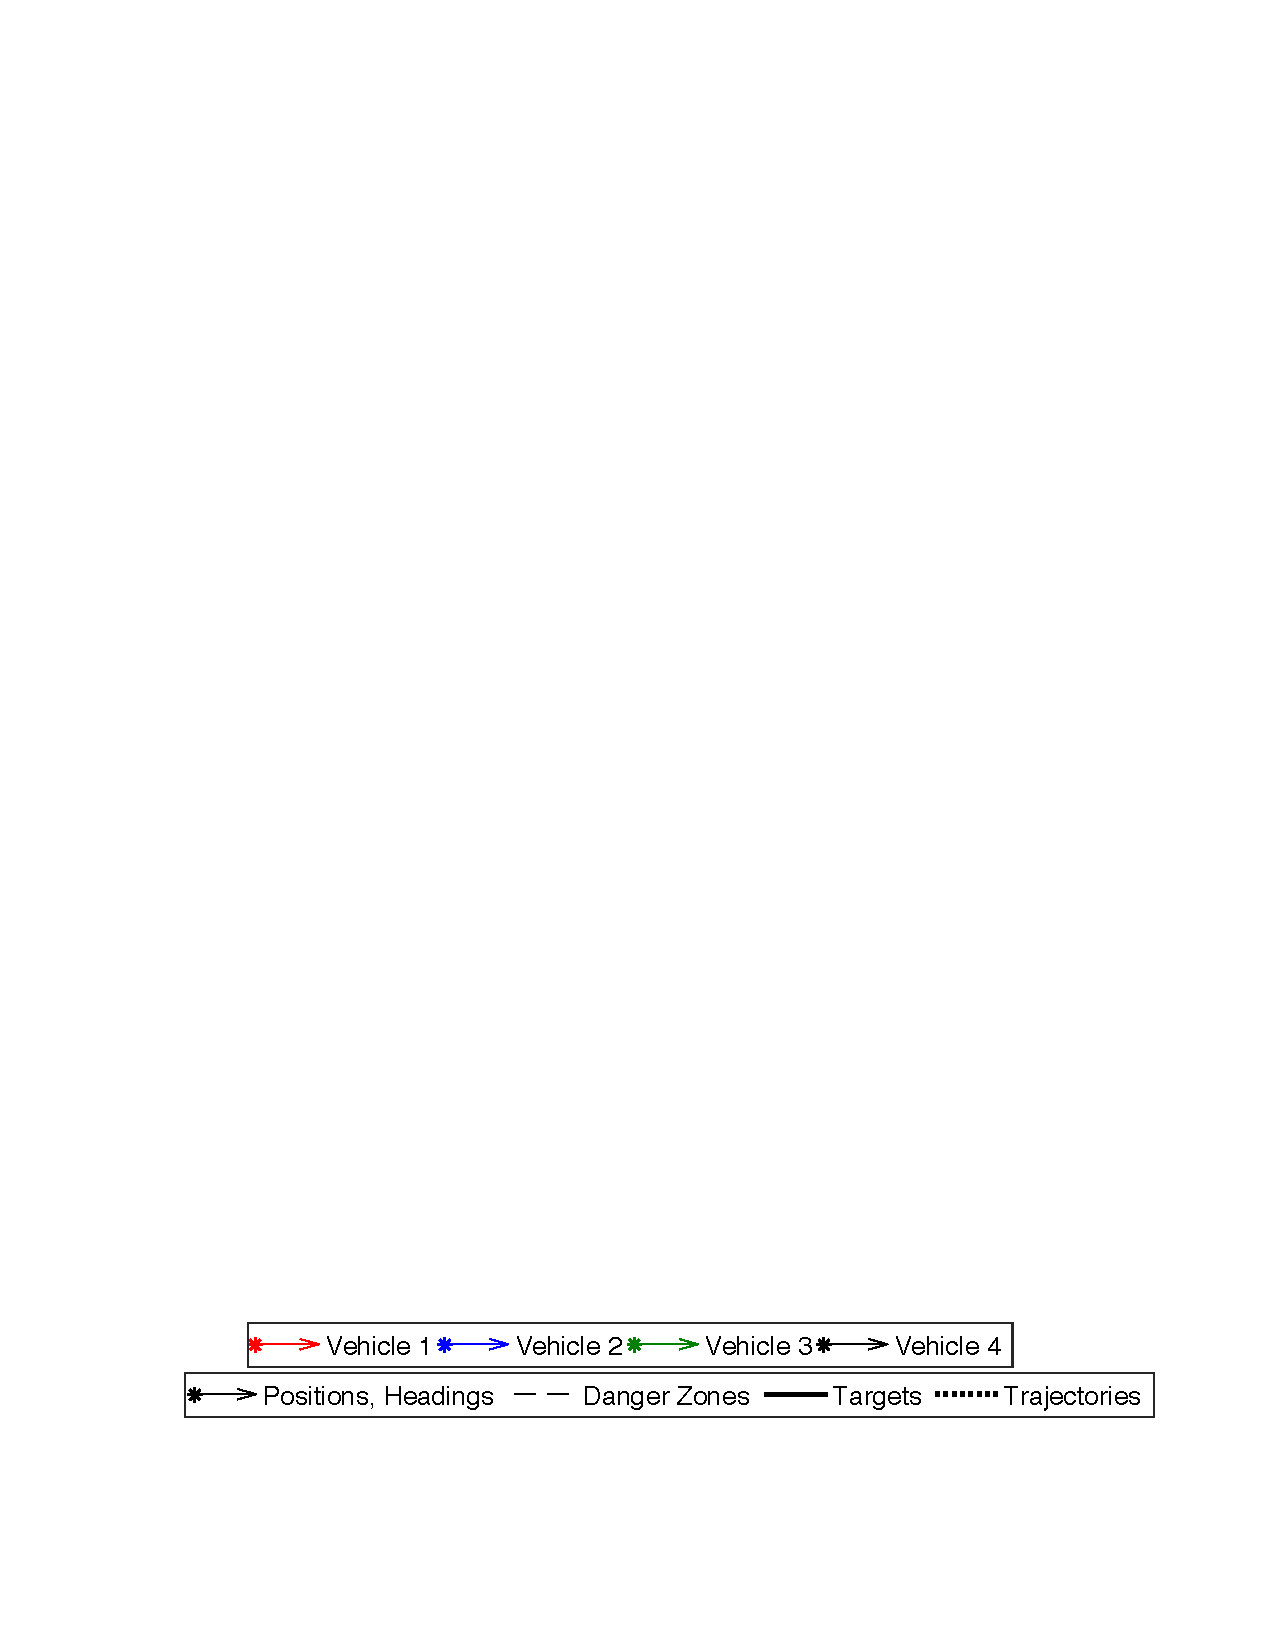
\includegraphics[width=\columnwidth]{fig/trajs_legend}
\end{subfigure}%
  \caption{Initial configuration and simulated trajectories of the vehicles for the three proposed methods.}
  \label{fig:allTrajs}
\end{figure}  

\begin{figure}[H]
  \centering
  \includegraphics[width=0.4\textwidth]{"fig/cc_rs3"}
  \caption{Evolution of the BRS and the obstacles induced by $\veh_1$ and $\veh_2$ for $\veh_3$ in the centralized control method.}
  \label{fig:cc_rs3}
\end{figure}
%%\vspace{-8em}
%
%\subsection{Centralized Control}
%\vspace{-1em}
%\begin{figure}[H]
%  \centering
%  \includegraphics[width=0.40\textwidth]{"fig/cc_traj"}
%  \caption{Simulated trajectories in the centralized control method. Since the higher priority vehicles induce relatively small obstacles in this case, vehicles do not deviate much from a straight line trajectory towards their respective targets.}
%  \label{fig:cc_traj}
%  \vspace{-1.4em}
%\end{figure}
%%\vspace{-4em}
Fig. \ref{fig:trajsCC} shows simulated trajectories in the situation where each vehicle uses $u^*_i(t, x_i)$ in \eqref{eq:opt_ctrl_i}. In this case, vehicles appear to deviate slightly from a straight line trajectory towards their targets, just enough to avoid higher-priority vehicles. The deviation is small since the centralized controller is quite restrictive, making the possible positions of higher-priority vehicles cover a small area. In the dense configuration at $t=-1.0$, the vehicles are close to each other but still outside each other's danger zones.

Fig. \ref{fig:cc_rs3} shows the evolution of the BRS for $\veh_3$ (green boundary), as well as the obstacles (black boundary) induced by the higher-priority vehicles. The size of the obstacles remains relatively small. $\ldt_i$ numbers for the four vehicles (in order) in this case are $-1.35, -1.37, -1.94$ and $-2.04$. They are relatively close for the vehicles, because the obstacles generated by higher-priority vehicles are small and hence do not affect $\ldt$ of the lower-priority vehicles significantly. 